% Options for packages loaded elsewhere
\PassOptionsToPackage{unicode}{hyperref}
\PassOptionsToPackage{hyphens}{url}
%
\documentclass[
]{article}
\usepackage{amsmath,amssymb}
\usepackage{iftex}
\ifPDFTeX
  \usepackage[T1]{fontenc}
  \usepackage[utf8]{inputenc}
  \usepackage{textcomp} % provide euro and other symbols
\else % if luatex or xetex
  \usepackage{unicode-math} % this also loads fontspec
  \defaultfontfeatures{Scale=MatchLowercase}
  \defaultfontfeatures[\rmfamily]{Ligatures=TeX,Scale=1}
\fi
\usepackage{lmodern}
\ifPDFTeX\else
  % xetex/luatex font selection
\fi
% Use upquote if available, for straight quotes in verbatim environments
\IfFileExists{upquote.sty}{\usepackage{upquote}}{}
\IfFileExists{microtype.sty}{% use microtype if available
  \usepackage[]{microtype}
  \UseMicrotypeSet[protrusion]{basicmath} % disable protrusion for tt fonts
}{}
\makeatletter
\@ifundefined{KOMAClassName}{% if non-KOMA class
  \IfFileExists{parskip.sty}{%
    \usepackage{parskip}
  }{% else
    \setlength{\parindent}{0pt}
    \setlength{\parskip}{6pt plus 2pt minus 1pt}}
}{% if KOMA class
  \KOMAoptions{parskip=half}}
\makeatother
\usepackage{xcolor}
\usepackage[margin=1in]{geometry}
\usepackage{color}
\usepackage{fancyvrb}
\newcommand{\VerbBar}{|}
\newcommand{\VERB}{\Verb[commandchars=\\\{\}]}
\DefineVerbatimEnvironment{Highlighting}{Verbatim}{commandchars=\\\{\}}
% Add ',fontsize=\small' for more characters per line
\usepackage{framed}
\definecolor{shadecolor}{RGB}{248,248,248}
\newenvironment{Shaded}{\begin{snugshade}}{\end{snugshade}}
\newcommand{\AlertTok}[1]{\textcolor[rgb]{0.94,0.16,0.16}{#1}}
\newcommand{\AnnotationTok}[1]{\textcolor[rgb]{0.56,0.35,0.01}{\textbf{\textit{#1}}}}
\newcommand{\AttributeTok}[1]{\textcolor[rgb]{0.13,0.29,0.53}{#1}}
\newcommand{\BaseNTok}[1]{\textcolor[rgb]{0.00,0.00,0.81}{#1}}
\newcommand{\BuiltInTok}[1]{#1}
\newcommand{\CharTok}[1]{\textcolor[rgb]{0.31,0.60,0.02}{#1}}
\newcommand{\CommentTok}[1]{\textcolor[rgb]{0.56,0.35,0.01}{\textit{#1}}}
\newcommand{\CommentVarTok}[1]{\textcolor[rgb]{0.56,0.35,0.01}{\textbf{\textit{#1}}}}
\newcommand{\ConstantTok}[1]{\textcolor[rgb]{0.56,0.35,0.01}{#1}}
\newcommand{\ControlFlowTok}[1]{\textcolor[rgb]{0.13,0.29,0.53}{\textbf{#1}}}
\newcommand{\DataTypeTok}[1]{\textcolor[rgb]{0.13,0.29,0.53}{#1}}
\newcommand{\DecValTok}[1]{\textcolor[rgb]{0.00,0.00,0.81}{#1}}
\newcommand{\DocumentationTok}[1]{\textcolor[rgb]{0.56,0.35,0.01}{\textbf{\textit{#1}}}}
\newcommand{\ErrorTok}[1]{\textcolor[rgb]{0.64,0.00,0.00}{\textbf{#1}}}
\newcommand{\ExtensionTok}[1]{#1}
\newcommand{\FloatTok}[1]{\textcolor[rgb]{0.00,0.00,0.81}{#1}}
\newcommand{\FunctionTok}[1]{\textcolor[rgb]{0.13,0.29,0.53}{\textbf{#1}}}
\newcommand{\ImportTok}[1]{#1}
\newcommand{\InformationTok}[1]{\textcolor[rgb]{0.56,0.35,0.01}{\textbf{\textit{#1}}}}
\newcommand{\KeywordTok}[1]{\textcolor[rgb]{0.13,0.29,0.53}{\textbf{#1}}}
\newcommand{\NormalTok}[1]{#1}
\newcommand{\OperatorTok}[1]{\textcolor[rgb]{0.81,0.36,0.00}{\textbf{#1}}}
\newcommand{\OtherTok}[1]{\textcolor[rgb]{0.56,0.35,0.01}{#1}}
\newcommand{\PreprocessorTok}[1]{\textcolor[rgb]{0.56,0.35,0.01}{\textit{#1}}}
\newcommand{\RegionMarkerTok}[1]{#1}
\newcommand{\SpecialCharTok}[1]{\textcolor[rgb]{0.81,0.36,0.00}{\textbf{#1}}}
\newcommand{\SpecialStringTok}[1]{\textcolor[rgb]{0.31,0.60,0.02}{#1}}
\newcommand{\StringTok}[1]{\textcolor[rgb]{0.31,0.60,0.02}{#1}}
\newcommand{\VariableTok}[1]{\textcolor[rgb]{0.00,0.00,0.00}{#1}}
\newcommand{\VerbatimStringTok}[1]{\textcolor[rgb]{0.31,0.60,0.02}{#1}}
\newcommand{\WarningTok}[1]{\textcolor[rgb]{0.56,0.35,0.01}{\textbf{\textit{#1}}}}
\usepackage{longtable,booktabs,array}
\usepackage{calc} % for calculating minipage widths
% Correct order of tables after \paragraph or \subparagraph
\usepackage{etoolbox}
\makeatletter
\patchcmd\longtable{\par}{\if@noskipsec\mbox{}\fi\par}{}{}
\makeatother
% Allow footnotes in longtable head/foot
\IfFileExists{footnotehyper.sty}{\usepackage{footnotehyper}}{\usepackage{footnote}}
\makesavenoteenv{longtable}
\usepackage{graphicx}
\makeatletter
\def\maxwidth{\ifdim\Gin@nat@width>\linewidth\linewidth\else\Gin@nat@width\fi}
\def\maxheight{\ifdim\Gin@nat@height>\textheight\textheight\else\Gin@nat@height\fi}
\makeatother
% Scale images if necessary, so that they will not overflow the page
% margins by default, and it is still possible to overwrite the defaults
% using explicit options in \includegraphics[width, height, ...]{}
\setkeys{Gin}{width=\maxwidth,height=\maxheight,keepaspectratio}
% Set default figure placement to htbp
\makeatletter
\def\fps@figure{htbp}
\makeatother
\setlength{\emergencystretch}{3em} % prevent overfull lines
\providecommand{\tightlist}{%
  \setlength{\itemsep}{0pt}\setlength{\parskip}{0pt}}
\setcounter{secnumdepth}{-\maxdimen} % remove section numbering
\ifLuaTeX
  \usepackage{selnolig}  % disable illegal ligatures
\fi
\usepackage{bookmark}
\IfFileExists{xurl.sty}{\usepackage{xurl}}{} % add URL line breaks if available
\urlstyle{same}
\hypersetup{
  pdftitle={Assignment 0 - Familiarity with Basic Data Wrangling and Modelling in R (Questions)},
  pdfauthor={GOV 1347 - Fall 2024},
  hidelinks,
  pdfcreator={LaTeX via pandoc}}

\title{Assignment 0 - Familiarity with Basic Data Wrangling and
Modelling in R (Questions)}
\author{GOV 1347 - Fall 2024}
\date{2024-08-24}

\begin{document}
\maketitle

This assignment is ungraded and is simply intended to give you a sense
of what we will be doing in class and to be sure you have all the tools
in place to successfully complete your blog posts. Whereas most of the
programming you will do in this course is very open-ended, this
assignment is designed to walk you step-by-step through some helpful
functions. You should complete this assignment after you have
successfully installed R/R Studio and set up your blog on GitHub. Feel
free to publish your responses to this assignment on your blog as a
test.

To get started, save this \texttt{.rmd} file and the data files
\texttt{state\_2pv\_1948\_2020.csv} and \texttt{nat\_pv\_1860\_2020.csv}
to the same directory (a folder) on your computer. We suggest creating a
directory specifically for this class, say ``Gov1347'' and then a
directory for each week, say ``Week1''. Whatever you call it, save your
\texttt{.rmd} and the data to the same location.

\textbf{Overview:} In this assignment, we will work with historical
national popular vote and state-level popular vote data from
presidential elections. We will restructure the two data sets and
eventually merge them, before running basic linear models to predict the
national popular vote from the vote in certain states.

\textbf{Data Details:}

\begin{itemize}
\item
  File Name: \texttt{state\_2pv\_1948\_2020.csv}
\item
  These data contain the state-level popular vote from presidential
  elections from 1948 through 2020.
\end{itemize}

\begin{longtable}[]{@{}
  >{\raggedright\arraybackslash}p{(\columnwidth - 2\tabcolsep) * \real{0.3559}}
  >{\raggedright\arraybackslash}p{(\columnwidth - 2\tabcolsep) * \real{0.6441}}@{}}
\toprule\noalign{}
\begin{minipage}[b]{\linewidth}\raggedright
Variable Name
\end{minipage} & \begin{minipage}[b]{\linewidth}\raggedright
Variable Description
\end{minipage} \\
\midrule\noalign{}
\endhead
\bottomrule\noalign{}
\endlastfoot
\texttt{year} & election year \\
\texttt{state} & state \\
\texttt{candidate} & candidate \\
\texttt{party} & candidate's party \\
\texttt{candidatevotes} & votes received by the candidate in the
state \\
\texttt{totalvotes} & total votes cast in the state \\
\texttt{vote\_share} & proportion of total votes received by the
candidate \\
\texttt{two\_party\_votes} & total votes cast for Republicans and
Democrats in the state \\
\texttt{two\_party\_vote\_share} & proportion of Democratic and
Republican votes received by the candidate \\
\end{longtable}

\begin{itemize}
\item
  File Name: \texttt{nat\_pv\_1860\_2020.csv}
\item
  These data contain the national-level popular vote from presidential
  elections from 1860 through 2020.
\end{itemize}

\begin{longtable}[]{@{}
  >{\raggedright\arraybackslash}p{(\columnwidth - 2\tabcolsep) * \real{0.3559}}
  >{\raggedright\arraybackslash}p{(\columnwidth - 2\tabcolsep) * \real{0.6441}}@{}}
\toprule\noalign{}
\begin{minipage}[b]{\linewidth}\raggedright
Variable Name
\end{minipage} & \begin{minipage}[b]{\linewidth}\raggedright
Variable Description
\end{minipage} \\
\midrule\noalign{}
\endhead
\bottomrule\noalign{}
\endlastfoot
\texttt{year} & election year \\
\texttt{npv\_democrat} & proportion of popular vote received by the
Democratic presidential candidate \\
\texttt{npv\_republican} & proportion of popular vote received by the
Republican presidential candidate \\
\end{longtable}

\section{Question 1: Loading Packages and
Data}\label{question-1-loading-packages-and-data}

\textbf{Loading packages:}

Once you install R and R Studio, you can open R Studio, which uses R in
the background. The first thing to do within RStudio is to install and
load the packages you will be using. You can read about packages and how
to install them on
\href{https://moderndive.netlify.app/1-getting-started.html\#packages}{Modern
Dive Section 1.3}. You will need two packages for this problem set:
\texttt{tidyverse} and \texttt{ggplot2}.
\footnote{One of the reasons R is such a widely used language is that there is a whole community that develops packages, which add functionality to the language. You can think of a package as just a collection of useful functions that aren't available in base R.}

The instructions at that link are primarily for the point-and-click
method of installing packages, but it's also important to know how to do
it via the command line. Some may find it easier as well. To install
packages via the command line, simply run
\texttt{install.packages("package\_name")} in RStudio, making sure the
package name is in quotes. Note that there are multiple ways to run a
command within RStudio: one way is to type the command in the
``Console'' pane of RStudio and press Return/Enter on your keyboard.
Another is to open a .Rmd file, create a code chunk, and press the green
play button in its top-right corner.

Once you install the packages, you can run
\texttt{library(package\_name)} to load it into RStudio. Note that the
package doesn't need to be in quotes inside the \texttt{library()}
function, but it can be if you like.

Load the packages \texttt{ggplot2} and \texttt{tidyverse} in the code
below.

\begin{Shaded}
\begin{Highlighting}[]
\FunctionTok{library}\NormalTok{(}\StringTok{"ggplot2"}\NormalTok{)}
\FunctionTok{library}\NormalTok{(}\StringTok{"tidyverse"}\NormalTok{)}
\end{Highlighting}
\end{Shaded}

\begin{verbatim}
## -- Attaching core tidyverse packages ------------------------ tidyverse 2.0.0 --
## v dplyr     1.1.4     v readr     2.1.5
## v forcats   1.0.0     v stringr   1.5.1
## v lubridate 1.9.3     v tibble    3.2.1
## v purrr     1.0.2     v tidyr     1.3.1
## -- Conflicts ------------------------------------------ tidyverse_conflicts() --
## x dplyr::filter() masks stats::filter()
## x dplyr::lag()    masks stats::lag()
## i Use the conflicted package (<http://conflicted.r-lib.org/>) to force all conflicts to become errors
\end{verbatim}

\textbf{Loading data:}

After loading the packages we need, it's time to read the data into R.
But there's one last step! Before you try to read data, it is a good
idea to tell R where on your computer you're working. To do that, you
need to set your working directory. Remember, ``directory'' is just a
computer science term for a folder on your computer. By setting your
working directory, you're telling R the folder in which to look for
files. Usually it's best practice to set your working directory to the
directory that your code is in. To do that, just go to the toolbar at
the top of your screen, select ``Session'', hover over ``Set Working
Directory'', and select ``To Source File Location''.

You can check your current working directory by running \texttt{getwd()}
with nothing in the parentheses. Try running \texttt{getwd()} in the
console to make sure your current working directory is the one where you
have this file saved. Make sure that you have downloaded the data for
this assignment into that same directory for the code below to work.
This works because by setting the working directory you told R the
folder where it will find the data.

Note: If you set the correct working directory but still get an error
running the code below, you may also need to click the downward arrow
next to the ``Knit'' button on the top of the ``Source'' pane and set
\texttt{Knit\ Directory} to either \texttt{Document\ Directory} or
\texttt{Current\ Working\ Directory}.

Load the data in the code chunk below:

\begin{Shaded}
\begin{Highlighting}[]
\NormalTok{nat }\OtherTok{\textless{}{-}} \FunctionTok{read\_csv}\NormalTok{(}\StringTok{"/Users/ellatrembanis/Desktop/Gov 1347/election{-}blog/election{-}blog/Week1/nat\_pv\_1860\_2020.csv"}\NormalTok{)}
\end{Highlighting}
\end{Shaded}

\begin{verbatim}
## Rows: 41 Columns: 3
## -- Column specification --------------------------------------------------------
## Delimiter: ","
## dbl (3): year, npv_democrat, npv_republican
## 
## i Use `spec()` to retrieve the full column specification for this data.
## i Specify the column types or set `show_col_types = FALSE` to quiet this message.
\end{verbatim}

\begin{Shaded}
\begin{Highlighting}[]
\NormalTok{state }\OtherTok{\textless{}{-}} \FunctionTok{read\_csv}\NormalTok{(}\StringTok{"/Users/ellatrembanis/Desktop/Gov 1347/election{-}blog/election{-}blog/Week1/state\_2pv\_1948\_2020.csv"}\NormalTok{)}
\end{Highlighting}
\end{Shaded}

\begin{verbatim}
## Rows: 1918 Columns: 10
## -- Column specification --------------------------------------------------------
## Delimiter: ","
## chr (3): state, candidate, party
## dbl (7): year, state_fips, candidatevotes, totalvotes, vote_share, two_party...
## 
## i Use `spec()` to retrieve the full column specification for this data.
## i Specify the column types or set `show_col_types = FALSE` to quiet this message.
\end{verbatim}

\section{Question 2: Transforming Data in the
Tidyverse}\label{question-2-transforming-data-in-the-tidyverse}

In this question, we will walk through a number of useful functions for
wrangling data in tidyverse: \texttt{select}, \texttt{arrange},
\texttt{mutate}, \texttt{filter}, and
\texttt{group\_by}/\texttt{summarize}. You are not by any means required
to use tidyverse in this course --- feel free to use base R if you are
more comfortable with it. But tidyverse has several data-wrangling tools
that are often more efficient and intuitive than base R.

\subsection{(a) Select}\label{a-select}

The \texttt{select} function is used when we want to focus on only
certain variables (i.e., columns) in our data set. There may be many
substantive reasons why we might want to remove certain columns, though
sometimes we may just want to remove columns to reduce clutter in the
data set. For the analysis we are conducting in this assignment, we do
not need the vote totals --- only two party vote share. Use the select
function to limit the state-level data set to only the variables
\texttt{year}, \texttt{state}, \texttt{party} and
\texttt{two\_party\_vote\_share}. Call this smaller dataframe
\texttt{state\_select}. Check the dimensions of the dataframe using the
\texttt{dim} function: it should have four columns and 1918 rows.

\begin{Shaded}
\begin{Highlighting}[]
\NormalTok{state\_select }\OtherTok{\textless{}{-}}\NormalTok{ state }\SpecialCharTok{|\textgreater{}}
  \FunctionTok{select}\NormalTok{(year, state, party, two\_party\_vote\_share)}
\FunctionTok{dim}\NormalTok{(state\_select)}
\end{Highlighting}
\end{Shaded}

\begin{verbatim}
## [1] 1918    4
\end{verbatim}

\subsection{(b) Arrange}\label{b-arrange}

The \texttt{arrange} function can be used to order the data set
according to a given variable. Right now, the \texttt{state\_select}
dataframe is in alphabetical order by state. Suppose that we want to
display the data set in order from most to least recent election. Use
the \texttt{arrange} function to order the data set by year. Use the
\texttt{head} function to ensure that elections from 2020 are indeed at
the top of the data set.

\emph{Hint: Consider wrapping the \texttt{year} variable in the
\texttt{desc()} function}

\begin{Shaded}
\begin{Highlighting}[]
\NormalTok{state\_select }\OtherTok{\textless{}{-}}\NormalTok{ state\_select }\SpecialCharTok{|\textgreater{}}
  \FunctionTok{arrange}\NormalTok{(}\FunctionTok{desc}\NormalTok{(year))}
\FunctionTok{head}\NormalTok{(state\_select)}
\end{Highlighting}
\end{Shaded}

\begin{verbatim}
## # A tibble: 6 x 4
##    year state   party      two_party_vote_share
##   <dbl> <chr>   <chr>                     <dbl>
## 1  2020 Alabama Democrat                   37.1
## 2  2020 Alabama Republican                 62.9
## 3  2020 Alaska  Democrat                   44.7
## 4  2020 Alaska  Republican                 55.3
## 5  2020 Arizona Democrat                   50.2
## 6  2020 Arizona Republican                 49.8
\end{verbatim}

\subsection{(c) Mutate}\label{c-mutate}

The \texttt{mutate} function allows you to define new variables or
redefine existing variables. Currently, the national data set only
includes the overall vote share of the parties (e.g., Democratic votes
divided by total votes). To be consistent with the state-level data,
define new variables \texttt{dem\_tpv} and \texttt{rep\_tpv} as the two
party vote share (as percentages) received by the Democratic and
Republican candidates, respectively. Then select only the \texttt{year},
\texttt{dem\_tpv}, and \texttt{rep\_tpv} columns and save this dataframe
as object \texttt{national\_mutate}.

\emph{Hint: the Democratic two party vote share is equal to Democratic
two party vote share divided by the Democratic two party vote share plus
the Republican two party vote share. You should multiply by 100 to get
vote shares as percentages.}

\begin{Shaded}
\begin{Highlighting}[]
\NormalTok{national\_mutate }\OtherTok{\textless{}{-}}\NormalTok{ nat }\SpecialCharTok{|\textgreater{}}
  \FunctionTok{mutate}\NormalTok{(}
    \AttributeTok{dem\_tpv =} \DecValTok{100}\SpecialCharTok{*}\NormalTok{npv\_democrat}\SpecialCharTok{/}\NormalTok{(npv\_democrat }\SpecialCharTok{+}\NormalTok{ npv\_republican),}
    \AttributeTok{rep\_tpv =} \DecValTok{100}\SpecialCharTok{*}\NormalTok{npv\_republican}\SpecialCharTok{/}\NormalTok{(npv\_democrat }\SpecialCharTok{+}\NormalTok{ npv\_republican)}
\NormalTok{  ) }\SpecialCharTok{|\textgreater{}}
  \FunctionTok{select}\NormalTok{(year, dem\_tpv, rep\_tpv)}
\FunctionTok{head}\NormalTok{(national\_mutate)}
\end{Highlighting}
\end{Shaded}

\begin{verbatim}
## # A tibble: 6 x 3
##    year dem_tpv rep_tpv
##   <dbl>   <dbl>   <dbl>
## 1  2020    52.2    47.8
## 2  2016    51.1    48.9
## 3  2012    52.0    48.0
## 4  2008    53.7    46.3
## 5  2004    48.8    51.2
## 6  2000    50.3    49.7
\end{verbatim}

\subsection{(d) Filter}\label{d-filter}

While the \texttt{select} function allows you to focus on certain
columns in a dataframe, the \texttt{filter} function allows you to focus
on certain rows. The state-level data set only includes data going back
to 1948, whereas the national data dates to 1860. Since we plan to merge
these data sets, use the \texttt{filter} function to subset your mutated
national data to only elections after 1948 (including 1948 itself). Save
this dataframe as \texttt{national\_mutate\_filter}.

\begin{Shaded}
\begin{Highlighting}[]
\NormalTok{national\_mutate\_filter }\OtherTok{\textless{}{-}}\NormalTok{ national\_mutate }\SpecialCharTok{|\textgreater{}}
  \FunctionTok{filter}\NormalTok{(year }\SpecialCharTok{\textgreater{}=} \DecValTok{1948}\NormalTok{)}
\end{Highlighting}
\end{Shaded}

\subsection{(e) Group\_by and Summarize}\label{e-group_by-and-summarize}

The \texttt{group\_by} and \texttt{summarize} functions are great for
quickly producing key summary information about your dataset. Suppose we
want to compare the average Democratic two party vote share in 21st
century elections between California and Massachusetts (note: consider
the 2000 election as part of the 21st century). Which state, in recent
years, has been more Democratic? Use the \texttt{filter} function to
subset the data set to 21st century elections \emph{and} subset the data
to only consider the Democratic vote share. Then, use \texttt{group\_by}
and \texttt{summarize} to get the average two party vote share by state.
Finally, use the \texttt{filter} function again to subset the summarized
data set to only California and Massachusetts.

\begin{Shaded}
\begin{Highlighting}[]
\NormalTok{state\_select }\SpecialCharTok{|\textgreater{}}
  \FunctionTok{filter}\NormalTok{(year }\SpecialCharTok{\textgreater{}=} \DecValTok{2000}\NormalTok{) }\SpecialCharTok{|\textgreater{}}
  \FunctionTok{filter}\NormalTok{(party }\SpecialCharTok{==} \StringTok{"Democrat"}\NormalTok{) }\SpecialCharTok{|\textgreater{}}
  \FunctionTok{group\_by}\NormalTok{(state) }\SpecialCharTok{|\textgreater{}}
  \FunctionTok{summarize}\NormalTok{(}
    \AttributeTok{avg\_dem\_share =} \FunctionTok{mean}\NormalTok{(two\_party\_vote\_share, }\AttributeTok{na.rm =}\NormalTok{ T)}
\NormalTok{  ) }\SpecialCharTok{|\textgreater{}}
  \FunctionTok{filter}\NormalTok{(state }\SpecialCharTok{==} \StringTok{"California"} \SpecialCharTok{|}\NormalTok{ state }\SpecialCharTok{==} \StringTok{"Massachusetts"}\NormalTok{)}
\end{Highlighting}
\end{Shaded}

\begin{verbatim}
## # A tibble: 2 x 2
##   state         avg_dem_share
##   <chr>                 <dbl>
## 1 California             61.1
## 2 Massachusetts          64.0
\end{verbatim}

Massachusetts has been more Democratic, on average, in 21st-century
presidential elections.

\section{Question 3: Pivoting Data: Wide to
Long}\label{question-3-pivoting-data-wide-to-long}

We're nearly ready to merge the national- and state-level data into a
single data frame. However, you may notice that the two data-frames
treat party differently. In the national data set, there are two
separate columns for two party vote (\texttt{dem\_tpv} and
\texttt{rep\_tpv}). This data structure is known as `'wide'' because
there are relatively more columns and fewer rows. The state-level data,
on the other hand, has a single column for two party vote and a separate
column (\texttt{party}) indicating whether the candidate is a Republican
or Democrat. This data structure is `'long'' because there are
relatively more rows and fewer columns. Use the \texttt{pivot\_longer}
function to convert the wide national data into the long format, and
call this new dataframe \texttt{national\_mutate\_filter\_long}.

\emph{Hint: After pivoting, this new dataframe should have three
columns: the year, the party, and the national two party vote share
(call this column \texttt{national\_two\_party\_vote\_share} or
similar). To make things consistent with the state-level data, use the
\texttt{mutate} function to make the \texttt{party} variable contain
entries of either `'Democrat'' or `'Republican.''}

\begin{Shaded}
\begin{Highlighting}[]
\NormalTok{national\_mutate\_filter\_long }\OtherTok{\textless{}{-}}\NormalTok{ national\_mutate\_filter }\SpecialCharTok{|\textgreater{}}
  \FunctionTok{pivot\_longer}\NormalTok{(}
    \AttributeTok{cols =} \FunctionTok{c}\NormalTok{(dem\_tpv, rep\_tpv),}
    \AttributeTok{names\_to =} \StringTok{"party"}\NormalTok{,}
    \AttributeTok{values\_to =} \StringTok{"national\_two\_party\_vote\_share"}
\NormalTok{  ) }\SpecialCharTok{|\textgreater{}}
  \FunctionTok{mutate}\NormalTok{(}
    \AttributeTok{party =} \FunctionTok{ifelse}\NormalTok{(party }\SpecialCharTok{==} \StringTok{"dem\_tpv"}\NormalTok{, }\StringTok{"Democrat"}\NormalTok{, }\StringTok{"Republican"}\NormalTok{)}
\NormalTok{  )}
\FunctionTok{head}\NormalTok{(national\_mutate\_filter\_long)}
\end{Highlighting}
\end{Shaded}

\begin{verbatim}
## # A tibble: 6 x 3
##    year party      national_two_party_vote_share
##   <dbl> <chr>                              <dbl>
## 1  2020 Democrat                            52.2
## 2  2020 Republican                          47.8
## 3  2016 Democrat                            51.1
## 4  2016 Republican                          48.9
## 5  2012 Democrat                            52.0
## 6  2012 Republican                          48.0
\end{verbatim}

\section{Question 4: Merging Data Sets:
Full\_Join}\label{question-4-merging-data-sets-full_join}

Finally, we're ready to merge the
\texttt{national\_mutate\_filter\_long} and \texttt{state\_select}
dataframes. Use the \texttt{full\_join} function to merge the two
dataframes by year and party.

Call this merged data set \texttt{combined\_data}. It should contain 5
columns: the state, party, year, two party vote share in the state, and
two party vote share for the candidate nationally.

\emph{Note that you could also use the \texttt{right\_join},
\texttt{left\_join}, or \texttt{inner\_join} here. In general, it is
usually safest to start with \texttt{full\_join} so that you don't
inadvertently eliminate rows in the data set. Suppose for example you
are trying to merge data sets by congressional district. If North
Dakota's lone district is called ND-01 in one dataframe and ND-AL in the
other, neither will be included in the joined dataframe if you use
\texttt{inner\_join}.}

\begin{Shaded}
\begin{Highlighting}[]
\NormalTok{combined\_data }\OtherTok{\textless{}{-}}\NormalTok{ national\_mutate\_filter\_long }\SpecialCharTok{|\textgreater{}}
  \FunctionTok{full\_join}\NormalTok{(state\_select, }\AttributeTok{by =} \FunctionTok{c}\NormalTok{(}\StringTok{"year"}\NormalTok{, }\StringTok{"party"}\NormalTok{))}
\FunctionTok{head}\NormalTok{(combined\_data)}
\end{Highlighting}
\end{Shaded}

\begin{verbatim}
## # A tibble: 6 x 5
##    year party    national_two_party_vote_share state      two_party_vote_share
##   <dbl> <chr>                            <dbl> <chr>                     <dbl>
## 1  2020 Democrat                          52.2 Alabama                    37.1
## 2  2020 Democrat                          52.2 Alaska                     44.7
## 3  2020 Democrat                          52.2 Arizona                    50.2
## 4  2020 Democrat                          52.2 Arkansas                   35.8
## 5  2020 Democrat                          52.2 California                 64.9
## 6  2020 Democrat                          52.2 Colorado                   56.9
\end{verbatim}

\section{Question 5: Pivoting Data: Long to
Wide}\label{question-5-pivoting-data-long-to-wide}

In the previous two questions, we pivoted the national data to a long
format and then merged the two data sets. Now, let's merge the data sets
in the wide format. Start with the \texttt{state\_select} dataframe and
use the \texttt{pivot\_wider} function so that that each column
represents the vote share \textbf{for a given party in a specific
state}. Call this dataframe \texttt{combined\_data\_wide}.

Merge this with the \texttt{national\_mutate\_filter} dataframe so that
you also have one column representing the national Democratic two party
vote proportion and one column representing the national Republican two
party vote proportion.

\emph{Hint: You should end up with 19 rows, one for each election year.
You should have 105 columns: the year, the national Democratic vote
share, the national Republican vote share, and the Democratic and
Republican vote shares in each of the 50 states + DC}

\begin{Shaded}
\begin{Highlighting}[]
\NormalTok{combined\_data\_wide }\OtherTok{\textless{}{-}}\NormalTok{ state\_select }\SpecialCharTok{|\textgreater{}}
  \FunctionTok{pivot\_wider}\NormalTok{(}
    \AttributeTok{names\_from =} \FunctionTok{c}\NormalTok{(}\StringTok{"party"}\NormalTok{, }\StringTok{"state"}\NormalTok{), }\AttributeTok{values\_from =} \FunctionTok{c}\NormalTok{(two\_party\_vote\_share)}
\NormalTok{  ) }\SpecialCharTok{|\textgreater{}}
  \FunctionTok{full\_join}\NormalTok{(national\_mutate\_filter, }\AttributeTok{by =} \StringTok{"year"}\NormalTok{)}
\FunctionTok{head}\NormalTok{(combined\_data\_wide)}
\end{Highlighting}
\end{Shaded}

\begin{verbatim}
## # A tibble: 6 x 105
##    year Democrat_Alabama Republican_Alabama Democrat_Alaska Republican_Alaska
##   <dbl>            <dbl>              <dbl>           <dbl>             <dbl>
## 1  2020             37.1               62.9            44.7              55.3
## 2  2016             35.6               64.4            41.6              58.4
## 3  2012             38.8               61.2            42.7              57.3
## 4  2008             39.1               60.9            38.9              61.1
## 5  2004             37.1               62.9            36.8              63.2
## 6  2000             42.4               57.6            32.1              67.9
## # i 100 more variables: Democrat_Arizona <dbl>, Republican_Arizona <dbl>,
## #   Democrat_Arkansas <dbl>, Republican_Arkansas <dbl>,
## #   Democrat_California <dbl>, Republican_California <dbl>,
## #   Democrat_Colorado <dbl>, Republican_Colorado <dbl>,
## #   Democrat_Connecticut <dbl>, Republican_Connecticut <dbl>,
## #   Democrat_Delaware <dbl>, Republican_Delaware <dbl>,
## #   `Democrat_District Of Columbia` <dbl>, ...
\end{verbatim}

\section{Question 6: Running Some Very Basic Linear
Models}\label{question-6-running-some-very-basic-linear-models}

\subsection{(a) Simple Regression}\label{a-simple-regression}

With the wide combined data set, run a basic linear model using the
\texttt{lm} function to predict the national two-party Democratic vote
share from the two party Democratic vote share in Florida. Interpret the
model coefficients and use the \texttt{summary} function to determine
whether the relationship is statistically significant.

\begin{Shaded}
\begin{Highlighting}[]
\NormalTok{lm1 }\OtherTok{\textless{}{-}} \FunctionTok{lm}\NormalTok{(dem\_tpv }\SpecialCharTok{\textasciitilde{}}\NormalTok{ Democrat\_Florida, }\AttributeTok{data =}\NormalTok{ combined\_data\_wide)}
\FunctionTok{summary}\NormalTok{(lm1)}
\end{Highlighting}
\end{Shaded}

\begin{verbatim}
## 
## Call:
## lm(formula = dem_tpv ~ Democrat_Florida, data = combined_data_wide)
## 
## Residuals:
##     Min      1Q  Median      3Q     Max 
## -4.9092 -1.2060 -0.0151  1.4236  9.1158 
## 
## Coefficients:
##                  Estimate Std. Error t value Pr(>|t|)    
## (Intercept)       20.4329     4.9123   4.160 0.000657 ***
## Democrat_Florida   0.6217     0.1044   5.953 1.57e-05 ***
## ---
## Signif. codes:  0 '***' 0.001 '**' 0.01 '*' 0.05 '.' 0.1 ' ' 1
## 
## Residual standard error: 3.208 on 17 degrees of freedom
## Multiple R-squared:  0.6758, Adjusted R-squared:  0.6568 
## F-statistic: 35.44 on 1 and 17 DF,  p-value: 1.572e-05
\end{verbatim}

\emph{Interpretation: The coefficient of 0.6217 means that for every one
percentage point increase in Democratic vote share in Florida, we would
expect the candidate to gain 0.6217 percentage points nationally. This
relationship is statistically significant, with a test statistic
approaching 6.}

\subsection{(b) Multiple Regression}\label{b-multiple-regression}

Now run a model predicting the national two-party Democratic vote share
from the two party Democratic vote share in Florida and New York. What
do you notice about the magnitude of the coefficient on the Florida term
relative to part (a)?

\begin{Shaded}
\begin{Highlighting}[]
\NormalTok{lm2 }\OtherTok{\textless{}{-}} \FunctionTok{lm}\NormalTok{(dem\_tpv }\SpecialCharTok{\textasciitilde{}}\NormalTok{ Democrat\_Florida }\SpecialCharTok{+} \StringTok{\textasciigrave{}}\AttributeTok{Democrat\_New York}\StringTok{\textasciigrave{}}\NormalTok{, }
           \AttributeTok{data =}\NormalTok{ combined\_data\_wide)}
\FunctionTok{summary}\NormalTok{(lm2)}
\end{Highlighting}
\end{Shaded}

\begin{verbatim}
## 
## Call:
## lm(formula = dem_tpv ~ Democrat_Florida + `Democrat_New York`, 
##     data = combined_data_wide)
## 
## Residuals:
##     Min      1Q  Median      3Q     Max 
## -2.8756 -1.0588 -0.1154  0.5401  6.1314 
## 
## Coefficients:
##                     Estimate Std. Error t value Pr(>|t|)    
## (Intercept)         13.73627    3.51341   3.910 0.001248 ** 
## Democrat_Florida     0.37573    0.08544   4.398 0.000449 ***
## `Democrat_New York`  0.32424    0.06710   4.833 0.000184 ***
## ---
## Signif. codes:  0 '***' 0.001 '**' 0.01 '*' 0.05 '.' 0.1 ' ' 1
## 
## Residual standard error: 2.108 on 16 degrees of freedom
## Multiple R-squared:  0.8682, Adjusted R-squared:  0.8517 
## F-statistic:  52.7 on 2 and 16 DF,  p-value: 9.101e-08
\end{verbatim}

\emph{Interpretation: The magnitude of the coefficient on the Florida
term is smaller than in the single-predictor model. This is likely due
to collinearities between Florida and New York: when they are both
included, Florida's individual explanatory power becomes diluted because
it is correlated with New York.}

These basic linear models are, of course, useless when it comes to
predicting the election result in advance of election day because we
only know the result in Florida or New York on election day (or
afterwards). These types of models could be more useful in trying to
determine the overall result of the election on election day; the New
York Times Needle, for example, updates its probabilities in real time
on election day as results come in (of course, these model are being fed
data at the county or precinct level, not just the state level). But the
very simple analysis above also touches on an important theme of the
course: election results are correlated across states. The Democratic
vote share in Florida is predictive of the national vote share, but it's
also predictive of the vote share in New York. And the correlation
between Florida and New York may be different than, for example, the
correlation between Florida and Georgia, given different demographics
and historical voting patterns.

\section{Question 7: Prediction}\label{question-7-prediction}

Using the multivariate model above, use the \texttt{predict} function to
predict the national two party Democratic vote share if the two party
Democratic vote share is 48\% in Florida and 60\% in New York.

\begin{Shaded}
\begin{Highlighting}[]
\NormalTok{test\_data }\OtherTok{\textless{}{-}} \FunctionTok{data.frame}\NormalTok{(}\AttributeTok{Democrat\_Florida =} \DecValTok{48}\NormalTok{, }\AttributeTok{Democrat\_New\_York =} \DecValTok{60}\NormalTok{) }\SpecialCharTok{|\textgreater{}}
  \FunctionTok{rename}\NormalTok{(}\StringTok{"Democrat\_New York"} \OtherTok{=}\NormalTok{ Democrat\_New\_York)}

\FunctionTok{predict}\NormalTok{(lm2, }\AttributeTok{newdata =}\NormalTok{ test\_data, }\AttributeTok{type =} \StringTok{"response"}\NormalTok{)}
\end{Highlighting}
\end{Shaded}

\begin{verbatim}
##        1 
## 51.22594
\end{verbatim}

\section{\texorpdfstring{Question 8: Saving \texttt{.csv}
Files}{Question 8: Saving .csv Files}}\label{question-8-saving-.csv-files}

The combined data sets you've created may be useful in the future, so
let's save them as \texttt{.csv} files to your directory so that you can
reuse them in future assignments using the \texttt{write.csv} function.

\begin{Shaded}
\begin{Highlighting}[]
\FunctionTok{write.csv}\NormalTok{(combined\_data\_wide, }\StringTok{"/Users/ellatrembanis/Desktop/Gov 1347/election{-}blog/election{-}blog/data/combined\_popular\_vote\_wide.csv"}\NormalTok{)}
\FunctionTok{write.csv}\NormalTok{(combined\_data, }\StringTok{"/Users/ellatrembanis/Desktop/Gov 1347/election{-}blog/election{-}blog/data/combined\_popular\_vote.csv"}\NormalTok{)}
\end{Highlighting}
\end{Shaded}

\section{Question 9: Visualization}\label{question-9-visualization}

\section{(a) Histogram}\label{a-histogram}

In \texttt{ggplot}, plot a histogram of the two-party Democratic vote
share in Florida going back to 1948 with \texttt{geom\_histogram}. Label
the chart as appropriate and play with different numbers of bins and
theme settings until you have a chart style you are satisfied with.

\begin{Shaded}
\begin{Highlighting}[]
\NormalTok{florida\_hist }\OtherTok{\textless{}{-}} \FunctionTok{ggplot}\NormalTok{(combined\_data\_wide, }
       \AttributeTok{mapping =} \FunctionTok{aes}\NormalTok{(}\AttributeTok{x =}\NormalTok{ Democrat\_Florida)) }\SpecialCharTok{+}
  \FunctionTok{geom\_histogram}\NormalTok{(}\AttributeTok{bins =} \DecValTok{20}\NormalTok{, }\AttributeTok{fill =} \StringTok{"darkblue"}\NormalTok{) }\SpecialCharTok{+}
  \FunctionTok{xlab}\NormalTok{(}\StringTok{"Two{-}Party Democratic Vote Share"}\NormalTok{) }\SpecialCharTok{+}
  \FunctionTok{ylab}\NormalTok{(}\StringTok{"Count"}\NormalTok{) }\SpecialCharTok{+}
  \FunctionTok{ggtitle}\NormalTok{(}\StringTok{"Democratic Performance in Florida Since 1948"}\NormalTok{)}
\NormalTok{florida\_hist}
\end{Highlighting}
\end{Shaded}

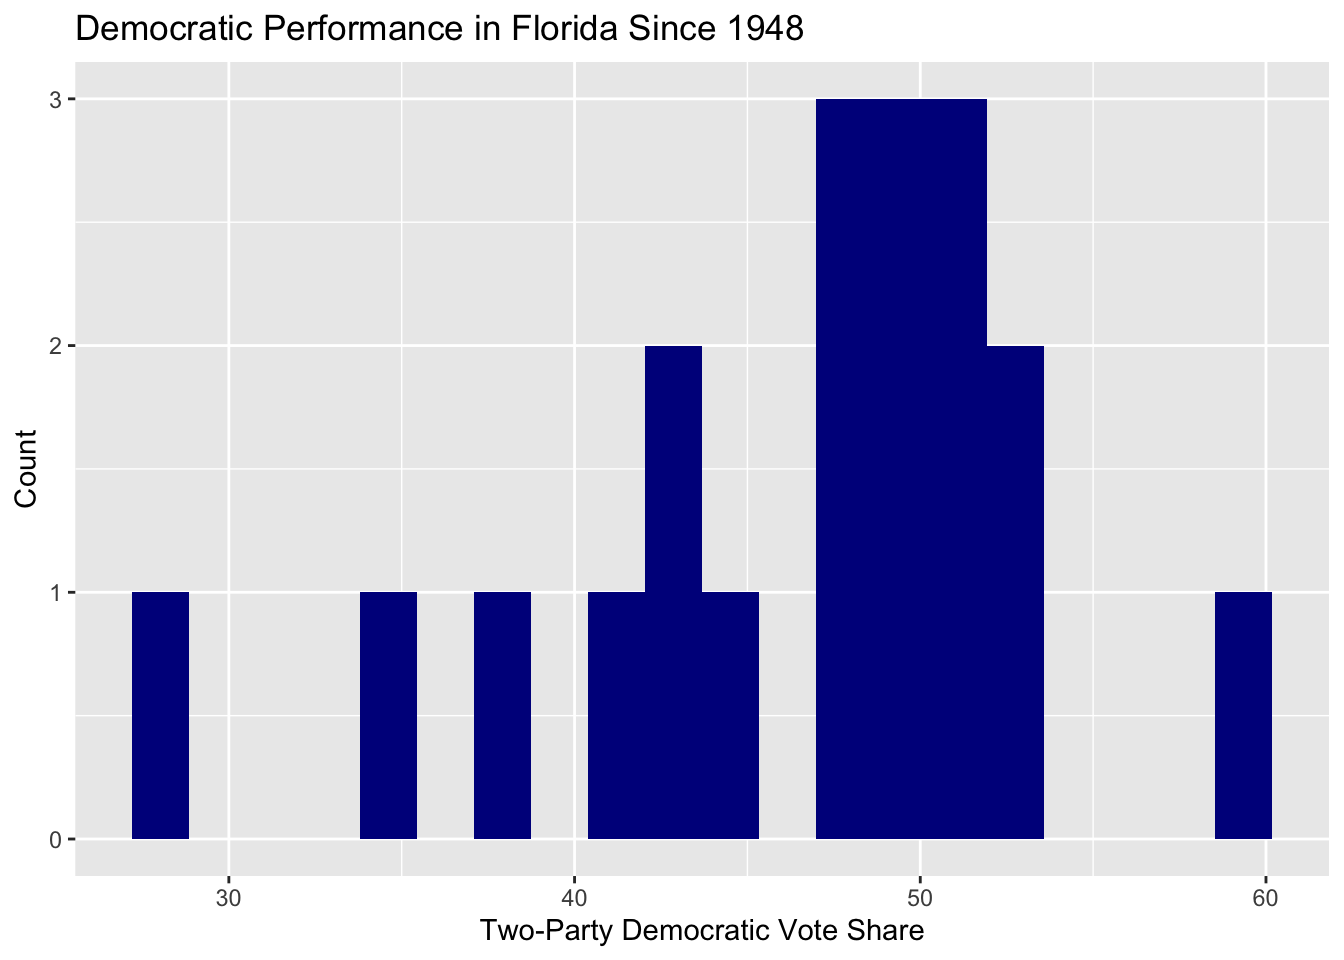
\includegraphics{Assignment_0_Questions_files/figure-latex/hist-1.pdf}

\begin{Shaded}
\begin{Highlighting}[]
\NormalTok{dem\_swing }\OtherTok{\textless{}{-}}\NormalTok{ combined\_data }\SpecialCharTok{|\textgreater{}}
  \FunctionTok{filter}\NormalTok{(party }\SpecialCharTok{==} \StringTok{"Democrat"}\NormalTok{) }\SpecialCharTok{|\textgreater{}}
  \FunctionTok{filter}\NormalTok{(state }\SpecialCharTok{==} \StringTok{"Georgia"} \SpecialCharTok{|}\NormalTok{ state }\SpecialCharTok{==} \StringTok{"Michigan"} \SpecialCharTok{|}\NormalTok{ state }\SpecialCharTok{==} \StringTok{"Arizona"} \SpecialCharTok{|}
\NormalTok{           state }\SpecialCharTok{==} \StringTok{"Wisconsin"} \SpecialCharTok{|}\NormalTok{ state }\SpecialCharTok{==} \StringTok{"Nevada"} \SpecialCharTok{|}\NormalTok{ state }\SpecialCharTok{==} \StringTok{"Pennsylvania"} \SpecialCharTok{|}
\NormalTok{           state }\SpecialCharTok{==} \StringTok{"North Carolina"}\NormalTok{)}

\NormalTok{state\_hist }\OtherTok{\textless{}{-}} \FunctionTok{ggplot}\NormalTok{(}\AttributeTok{data =}\NormalTok{ dem\_swing, }
                     \AttributeTok{mapping =} \FunctionTok{aes}\NormalTok{(}\AttributeTok{x =}\NormalTok{ two\_party\_vote\_share)) }\SpecialCharTok{+}
  \FunctionTok{geom\_histogram}\NormalTok{(}\AttributeTok{bins =} \DecValTok{20}\NormalTok{, }\AttributeTok{fill =} \StringTok{"darkblue"}\NormalTok{) }\SpecialCharTok{+}
  \FunctionTok{facet\_wrap}\NormalTok{(}\SpecialCharTok{\textasciitilde{}}\NormalTok{ state) }\SpecialCharTok{+}
  \FunctionTok{xlab}\NormalTok{(}\StringTok{"Two{-}Party Democratic Vote Share"}\NormalTok{) }\SpecialCharTok{+}
  \FunctionTok{ylab}\NormalTok{(}\StringTok{"Count"}\NormalTok{) }\SpecialCharTok{+}
  \FunctionTok{ggtitle}\NormalTok{(}\StringTok{"Democratic Performance Since 1948 In 2024 Swing States"}\NormalTok{) }\SpecialCharTok{+}
  \FunctionTok{geom\_vline}\NormalTok{(}\AttributeTok{xintercept =} \DecValTok{50}\NormalTok{)}
\NormalTok{state\_hist}
\end{Highlighting}
\end{Shaded}

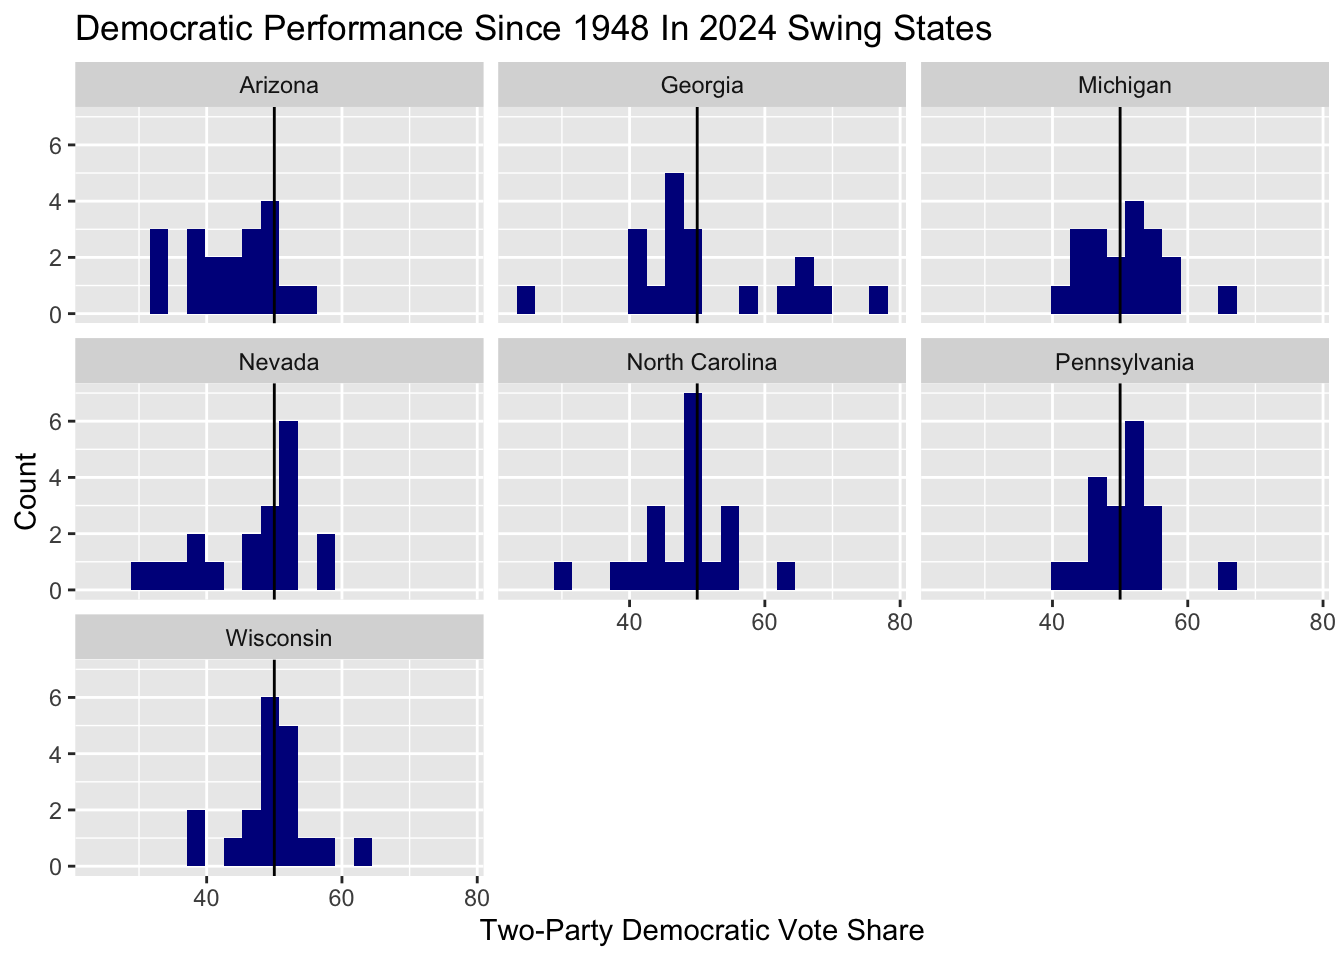
\includegraphics{Assignment_0_Questions_files/figure-latex/facet wrap-1.pdf}
\#\# (b) Scatterplot In ggplot, plot a scatterplot of the two-party
Democratic vote share in Florida going back to 1948 on the x-axis and
the national Democratic two-party vote share on the y-axis. Instead of
dots, label each point with the election year using geom\_label. Also
label the chart as appropriate and play with different theme settings
until you have a chart style you are satisfied with.

\begin{Shaded}
\begin{Highlighting}[]
\NormalTok{florida\_scatter }\OtherTok{\textless{}{-}} \FunctionTok{ggplot}\NormalTok{(combined\_data\_wide, }
                          \AttributeTok{mapping =} \FunctionTok{aes}\NormalTok{(}\AttributeTok{x =}\NormalTok{ Democrat\_Florida, }\AttributeTok{y =}\NormalTok{ dem\_tpv,}
                                        \AttributeTok{label =}\NormalTok{ year)) }\SpecialCharTok{+}
  \FunctionTok{geom\_label}\NormalTok{() }\SpecialCharTok{+}
  \FunctionTok{xlab}\NormalTok{(}\StringTok{"Two{-}Party Democratic Vote Share in Florida"}\NormalTok{) }\SpecialCharTok{+}
  \FunctionTok{ylab}\NormalTok{(}\StringTok{"Two{-}Party National Democratic Vote Share"}\NormalTok{) }\SpecialCharTok{+}
  \FunctionTok{ggtitle}\NormalTok{(}\StringTok{"Democratic Performance in Florida vs. National Vote Share"}\NormalTok{)}
\NormalTok{florida\_scatter}
\end{Highlighting}
\end{Shaded}

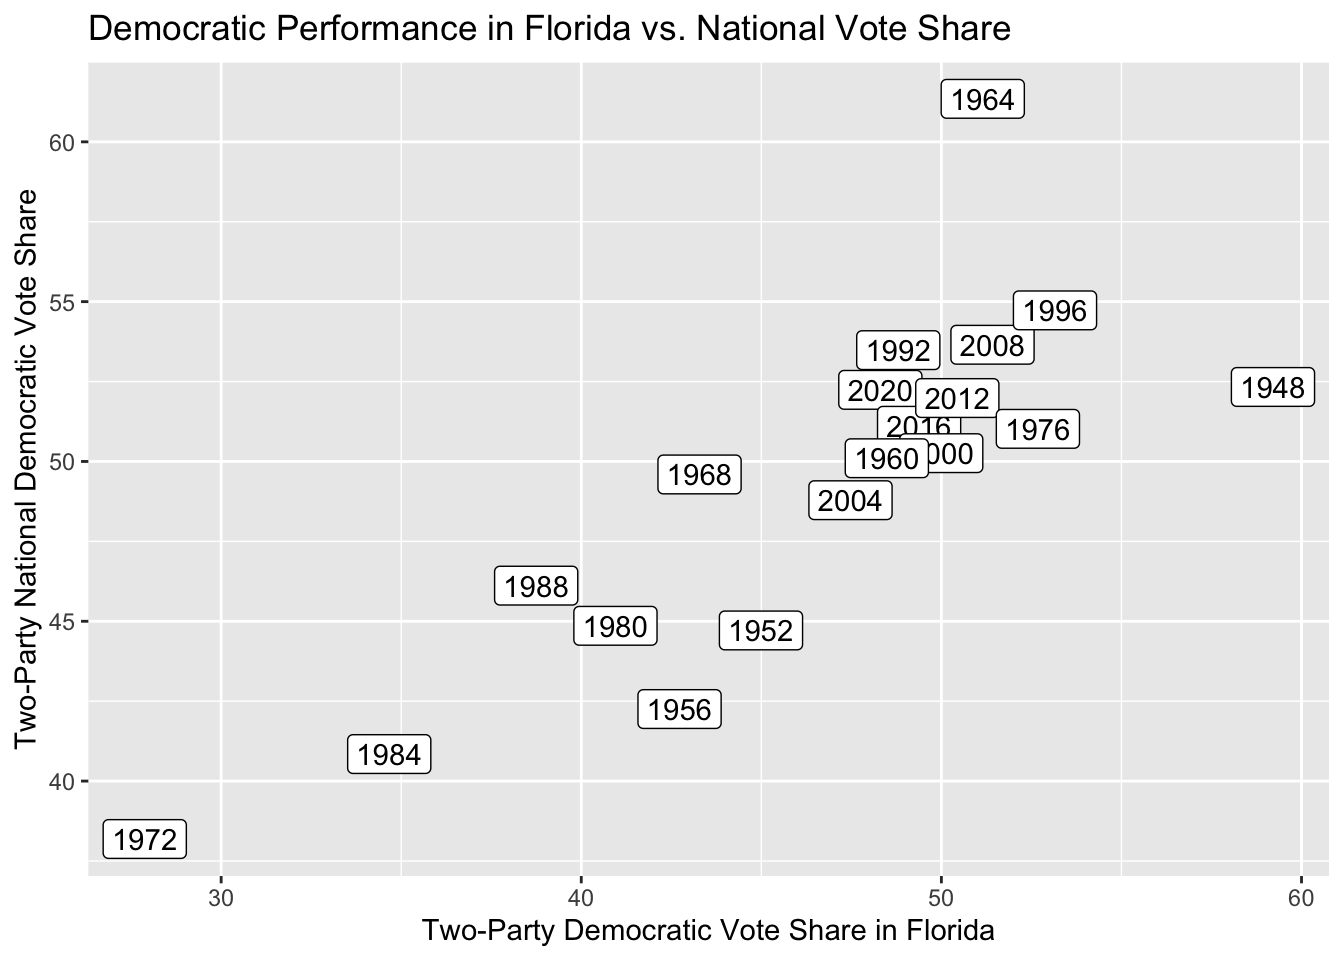
\includegraphics{Assignment_0_Questions_files/figure-latex/scatter-1.pdf}

\end{document}
